\section{Unemployment}
\subsection{Efficiency Wages}

\paragraph{Assumptions}
\begin{align*}
y _ { i} = A _ { i } \cdot f \left( \ell _ { i } \right)
&&
\Phi = 0
&&
\ell _ { i } = \ell N _ { i }
&&
TC  = wN_i 
&&
A_i = A
\end{align*}

Monopsony over job positions:
\begin{align*}
y = nm y_i = A f(eN)
&&
TC = wN
&&
p_j = P
\end{align*}

We can write the profit function of the individual firm as:

\begin{equation*}
    \pi=\frac{\pi}{P}=\frac{p_{j}}{P}y-\frac{w}{P}N=y-\omega.N=Af(e.N)-\omega.N
\end{equation*}

The problem of the firm is that of maximizing their profits, choosing the number of workers, and on the real wages to pay them. Formalizing this: 
\begin{equation*}
\begin{aligned}
    \underset{N,\omega}{max} \pi=Af(e.N)-\omega.N \\
   \text{subjecto to} && e=e(\omega) && e'(.)=0
\end{aligned}
\end{equation*}

The $e$ in this problem is a function that measures worker effort, given the real wage they are being paid. There are 5 main foundations for this type of behaviour: 
\begin{itemize}
    \item Biological
    \item Heterogeneity
    \item Sociological
    \item Economical 
    \item Strategic reasons
\end{itemize}

Let us see the first order conditions for the maximization problem of the firm, 
\begin{equation*}
    \frac{\partial\pi}{\partial N}= 0 \implies A.e.f'-\omega=0 \implies A.f'(e.N)=\frac{\omega}{e}
\end{equation*}
We can easily identify that $A.f'(e.N)$ is the marginal productivity of labour, and $\tfrac{\omega}{e}$ is the real wage per unit of effort. 

\begin{equation*}
    \frac{\partial\pi}{\partial N}=o \implies A.N.f'.e'-N=0 \implies af'(e.N)=\frac{1}{e'(\omega)}
\end{equation*}

Putting both F.O.C together we get:
\begin{equation*}
    \frac{1}{e'(\omega)}=\frac{\omega}{e} \implies \frac{de}{d\omega}\frac{\omega}{e}=1    
\end{equation*}

$\frac{de}{d\omega}\frac{\omega}{e}=1$ is known as the Solow condition. Note the left-hand side of the equation is the elasticity of effort with respect to the real wage. 

\subsubsection{A model based on Shapiro and Stiglitz (1983) (Non-Shirking)}

The production function comes as $y=A.\ell^{\beta}$ where $\ell=e.N$. E is defined as one of two conditions, either the worker is actually working hard, or he's not putting any effort at all, so $e$ is defined as: 

\[
e= \left\{
    \begin{array}{l l}
         \overline{e} & \omega\geq\omega_{0} \\
         0  & \omega<\omega_{0}
    \end{array}
\right.
\]

Note also, $\overline{e}<1$.

\begin{figure}[H]
    \centering
    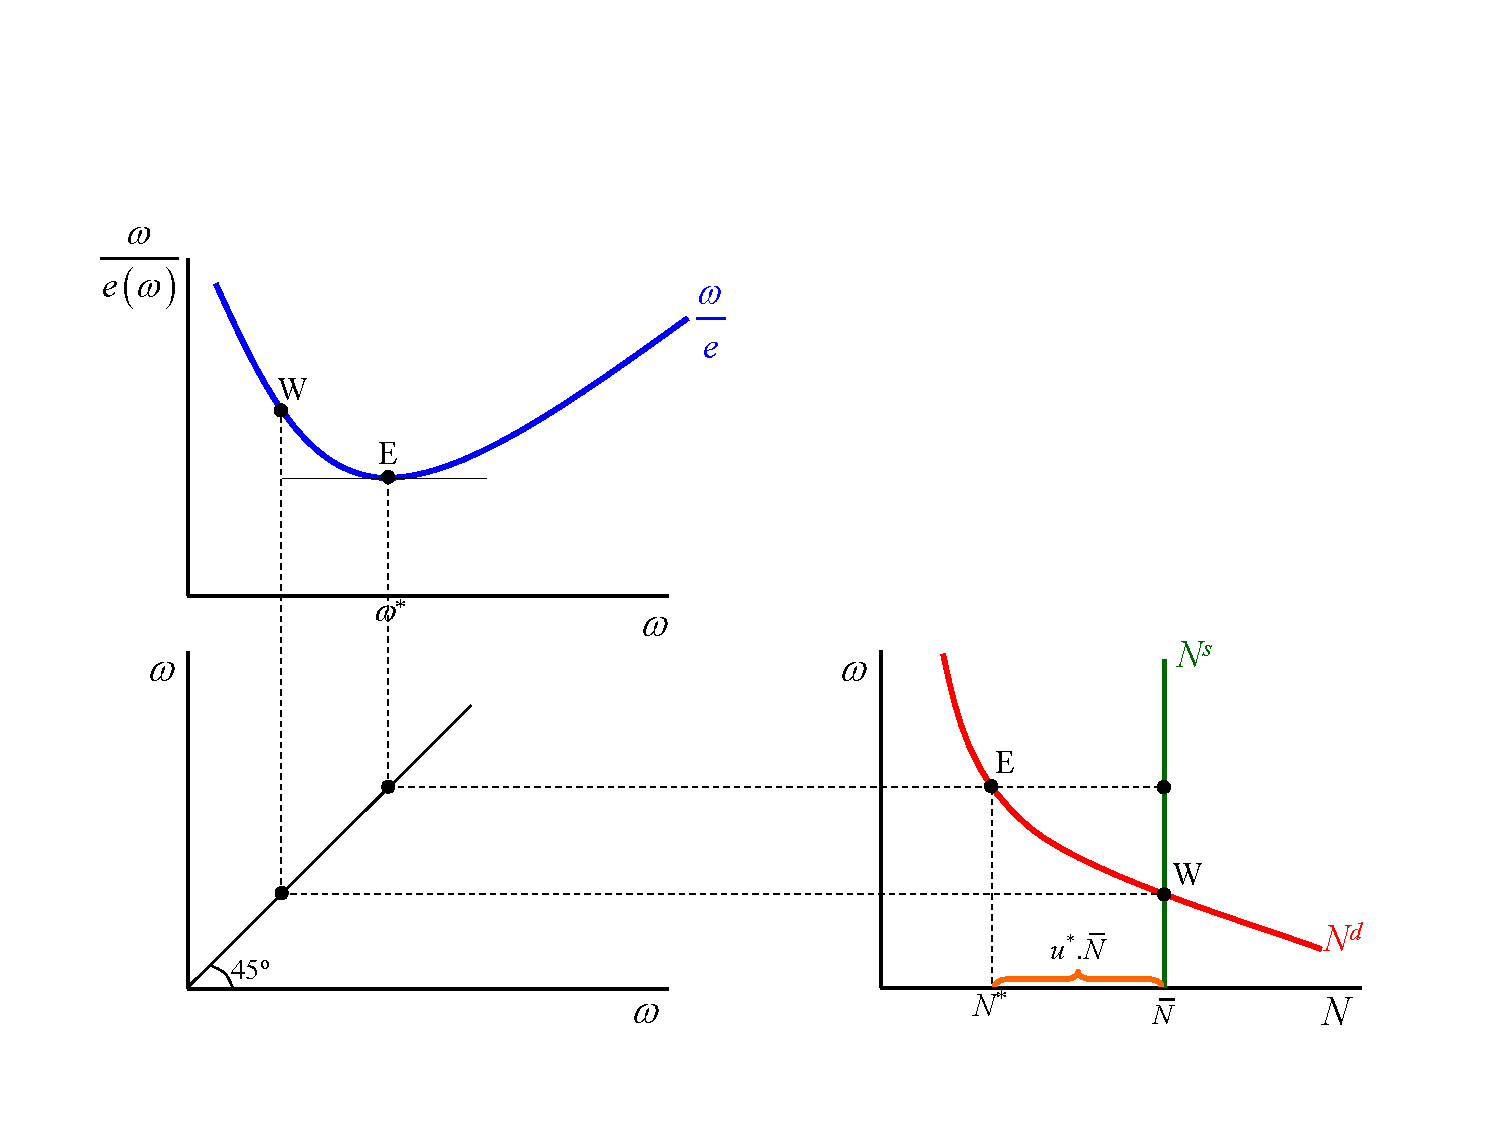
\includegraphics[max width=\linewidth]{4_0_New_Keynesian_School/efficiency_wages_graph.pdf}
    \caption{Efficiency wages and involuntary unemployment}  
\end{figure}
\paragraph{A static model of effort supply faced by the firm}

Utility: $U=C^{\alpha}(1-e)^{1-\alpha}$ \\

Consumption: $C=B(1-S)+S\omega$

Where 
\[
S=\left\{
\begin{array}{ll}
      1 & \text{If employed} \\
      0 & \text{If unemployed}\\

\end{array} 
\right. \]

And B is the employment benefit, defined as $B< max(\omega ,\omega    (1-e)^{\frac{1-\alpha}{\alpha}})$. 
The following table summarizes the consumption, leisure, and utility for each individual, depending on their employment status.

\begin{table}[H]
\begin{tabu} to \linewidth{|X[-2.5,c,m]|X[c,m]|X[c,m]|X[c,m]|}
\tabucline-
   Individual & Consumption (C) & Leisure (Z) & Utility(U)  \\ \hline
    Non-Shirker (N) & $\omega$ & $1-\overline{e}$ & $U_{S}=\omega^{\alpha}(1-\overline{e})^{1-\alpha}$ \\ \hline
    Shirker (S) & $\omega$ & 1-0 & $U_{N}=\omega^{\alpha}$  \\ \hline
    Unemployed(U) & B & 1-0 & $U_{U}=B^{\alpha}$\\
    \hline
\end{tabu}
\caption{Outcomes for participants}
\end{table}

Note $U_{U}<U_{N}<U_{S}$.

\begin{itemize}
    \item $0 \leq u \leq 1$ is the unemployment rate, i.e. the probability of not finding a new job. 
    \item $0\leq q \leq 1$ is the probability of being caught shirking 
\end{itemize}


\begin{figure}[ht]

\centering
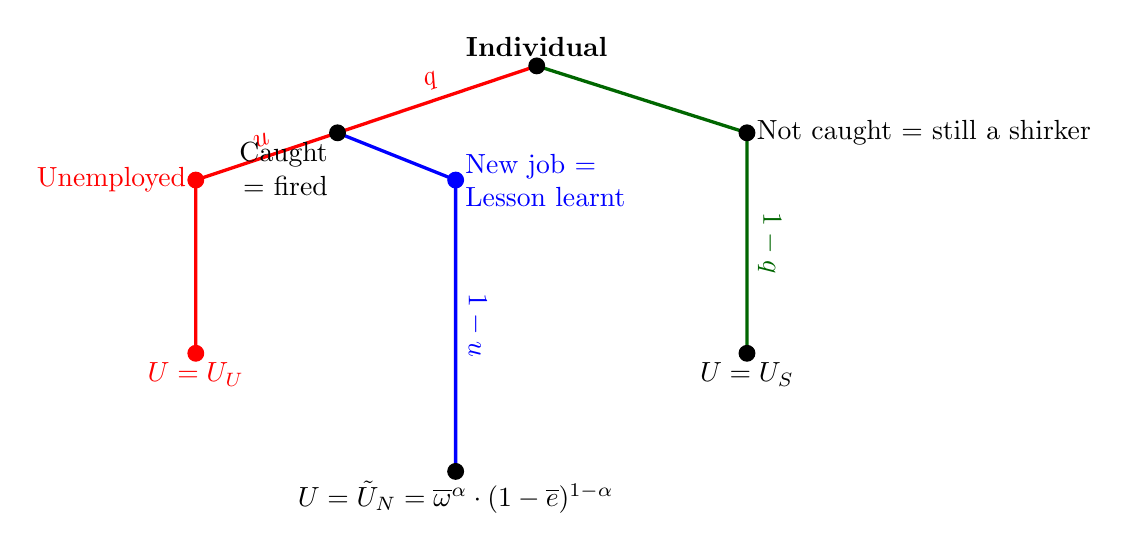
\begin{tikzpicture}[scale=1]


\coordinate (a) at (3.83, 2.65);
\coordinate (c) at (1.3, 1.8);
\coordinate (d) at (2.8, -2.5);
\coordinate (e) at (-0.5,-1);
\coordinate (f) at (6.5, -1);
\coordinate (g) at (-0.5, 1.2);
\coordinate (h) at (2.8, 1.2);



\draw [very thick, red] (e) -- (g) -- (c) node[pos=0.5,sloped,above] {$u$};
\draw [very thick, red] (a) -- (c) node[pos=0.5,sloped,above] {$q$}; 




\draw [very thick, black!60!green] (a) -- (6.5, 1.8) -- (f) node[pos=0.5,sloped,above] {$1-q$};



\draw [very thick, blue] (c) -- (h) -- (d) node[pos=0.5,sloped,above] {$1-u$};


\draw [fill] (c) circle [radius=0.1] node [below left, align = right] {Caught \\ = fired};
\draw [fill] (6.5, 1.8) circle [radius=0.1] node  [right] {Not caught = still a shirker};
\draw [fill = black] (a) circle [radius=0.1] node [above] {\textbf{Individual}};
\draw [fill] (d) circle [radius=0.1] node [below] {$U = \tilde { U } _ { N } = \overline { \omega } ^ { \alpha } \cdot ( 1 - \overline { e } ) ^ { 1 - \alpha }$};
\draw [fill, red] (e) circle [radius=0.1] node [below] { $U = U_U$};
\draw [fill] (f) circle [radius=0.1] node [below] {$U = U_S$};
\draw [fill, red] (g) circle [radius=0.1] node [left] {Unemployed};
\draw [fill, blue, align = left] (h) circle [radius=0.1] node [right] {New job = \\ Lesson learnt};

\end{tikzpicture}
\caption{Decision tree for a shirker}
\end{figure}



\begin{equation*}
\begin{aligned}
    E(U_{S})=q[(1-u).\Tilde{U}_{N}+u.U_{U}]+(1+q)U_{S} \\
  &&& \texttt{Where} &&& \overline{V}=(1-u).\Tilde{U}_{N}+uU_{U} \\
\end{aligned}
\end{equation*}

\begin{equation*}
\begin{aligned}
    \overline{V}=(1-u)[\overline{\omega}^{\alpha}(1-\overline{e})^{1-\alpha}]+uB^{\alpha} \\
    q.\overline{V}+(1-q)\omega^{\alpha}=\omega^{\alpha}.\overline{V}(1-\overline{e})^{1-\alpha}
\end{aligned}
\end{equation*}

Note that $E(U_{S}\leq U_{N}$. Replacing $\overline{V}$ in $E(U_{S})$: 

\begin{equation*}
    q.\overline{V}+(1-q)\omega^{\alpha}=\omega^{\alpha}.\overline{V}(1-\overline{e}^{1-\alpha}
\end{equation*}

Solving for $\omega$ we get the No-Shirking Condition for an individual firm: 

\begin{equation}\label{NSC_firm}
    \omega=\bigg[ \frac{q.\overline{V}}{(1-\overline{e})^{1-\alpha-(1-q)}} \bigg]
\end{equation}
By assumption, $q>1-(1-\overline{e})^{1-\alpha}$ \\
To see the NSC graphically: 

\begin{figure}[H]
\centering
\begin{tikzpicture}[scale=1.5]

% Axis

\draw [ultra thick](0,0) -- (8,0);

\draw [ultra thick](0,0) -- (0,5.5);

\node [left] at (-0.2,5.3) {$\omega$};
\node [below left] at (0,0) {$0$};

\node [below] at (8.2,-0.2) {$1 - u$};

\node [left] at (0,1) {$\left[ \frac { q B ^ { \alpha } } { ( 1 - \overline { e } ) ^ { 1 - \alpha } - ( 1 - q ) } \right] ^ { \frac { 1 } { \alpha } }$};


\node [left] at (0,3.5) {$\left[ \frac { q \cdot \overline { \omega } ^ { \alpha } \cdot ( 1 - \overline { e } ) ^ { 1 - \alpha } } { ( 1 - \overline { e } ) ^ { 1- \alpha } - ( 1 - q ) } \right] ^ { \frac { 1 } { \alpha } }$};

%Curve
\draw[very thick, blue] (0,1) to [out=5,in=220]  (6,3.5) node[right]{$NSC_i$};
\draw [dashed] (0,3.5) -- (6,3.5);
\draw [dashed] (6,5)--(6,0)node[below]{$1$};
\end{tikzpicture}

\caption{NSC for an individual firm}

\end{figure}


\begin{equation*}
    \Tilde{U}_{N}>U_{U} \implies \frac{\partial\overline{V}}{\partial(1-u)>0}\implies \frac{\partial\omega}{\partial(1-u)}>0
\end{equation*}

From here we can derive the macroeconomic No-Shirking Condition:

\begin{equation}\label{NSC_macro}
    \omega=\bigg[\frac{quB^{\alpha}}{(1-\overline{e})^{1-\alpha}[1-q(1-u)]-(1-q)} \bigg]
\end{equation}

\begin{figure}[H]
\centering
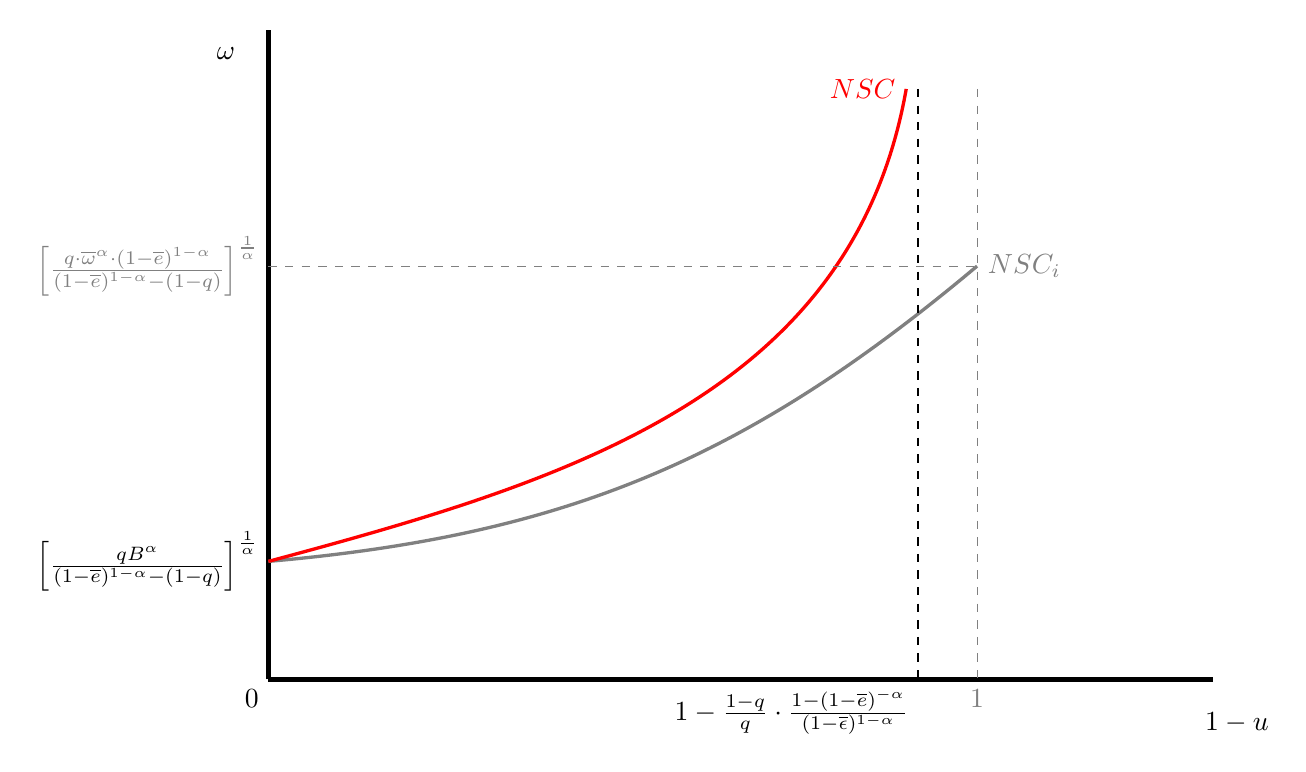
\begin{tikzpicture}[scale=1.5]

% Axis

\draw [ultra thick](0,0) -- (8,0);

\draw [ultra thick](0,0) -- (0,5.5);

\node [left] at (-0.2,5.3) {$\omega$};

\node [below] at (8.2,-0.2) {$1 - u$};
\node [below left] at (0,0) {$0$};

\node [left] at (0,1) {$\left[ \frac { q B ^ { \alpha } } { ( 1 - \overline { e } ) ^ { 1 - \alpha } - ( 1 - q ) } \right] ^ { \frac { 1 } { \alpha } }$};


\node[gray] [left] at (0,3.5) {$\left[ \frac { q \cdot \overline { \omega } ^ { \alpha } \cdot ( 1 - \overline { e } ) ^ { 1 - \alpha } } { ( 1 - \overline { e } ) ^ { 1- \alpha } - ( 1 - q ) } \right] ^ { \frac { 1 } { \alpha } }$};

%Curve
\draw[very thick, gray] (0,1) to [out=5,in=220]  (6,3.5) node[right]{$NSC_i$};
\draw[very thick, red] (0,1) to [out=15,in=260]  (5.4,5) node[left]{$NSC$};

\draw [dashed, gray] (0,3.5) -- (6,3.5);
\draw [dashed, gray] (6,5)--(6,0)node[below]{$1$};
\draw [dashed] (5.5,5)--(5.5,0)node[below left]{$1 - \frac { 1 - q } { q } \cdot \frac { 1 - ( 1 - \overline { e } ) ^ { - \alpha } } { ( 1 - \overline { \epsilon } ) ^ {1 - \alpha } }$};
\end{tikzpicture}

\caption{Macroeconomic NSC}

\end{figure}

This is just one side of the equilibrium, however, so we must calculate a labour demand in order to achieve an actual equilibrium. 
\begin{equation}\label{Inv_Labour_Demand}
    Af'(L)=\frac{\omega}{\overline{e}} \implies \omega=\overline{e}Af'\big[\overline{e}(1-u)\overline{N}\big]
\end{equation}
This is the inverse labour demand for employees. Note that it is decreasing because the marginal productivity of labour is decreasing as well. 


\begin{equation*}
 \left. \omega \right\rvert_{NSC} = \bigg[\frac{q.u}{Z(u,q)}\bigg]^{\frac{1}{\alpha}}B 
\end{equation*}

We can see the relation of the real wage to the unemployment rate, the employment benefits, and the probability of being caught shirking, as the derivatives of the last equation, 

\begin{equation*}
    \begin{aligned}
        \frac{\partial\left. \omega \right\rvert_{NSC}}{\partial u}<0 \\
        \frac{\partial\left. \omega \right\rvert_{NSC}}{\partial B}>0 \\
        \frac{\partial\left. \omega \right\rvert_{NSC}}{\partial q}<0
    \end{aligned}
\end{equation*}

To wrap up, comes the graphic for the equilibrium, and the effect of shocks: 
\begin{figure}[H]
\centering
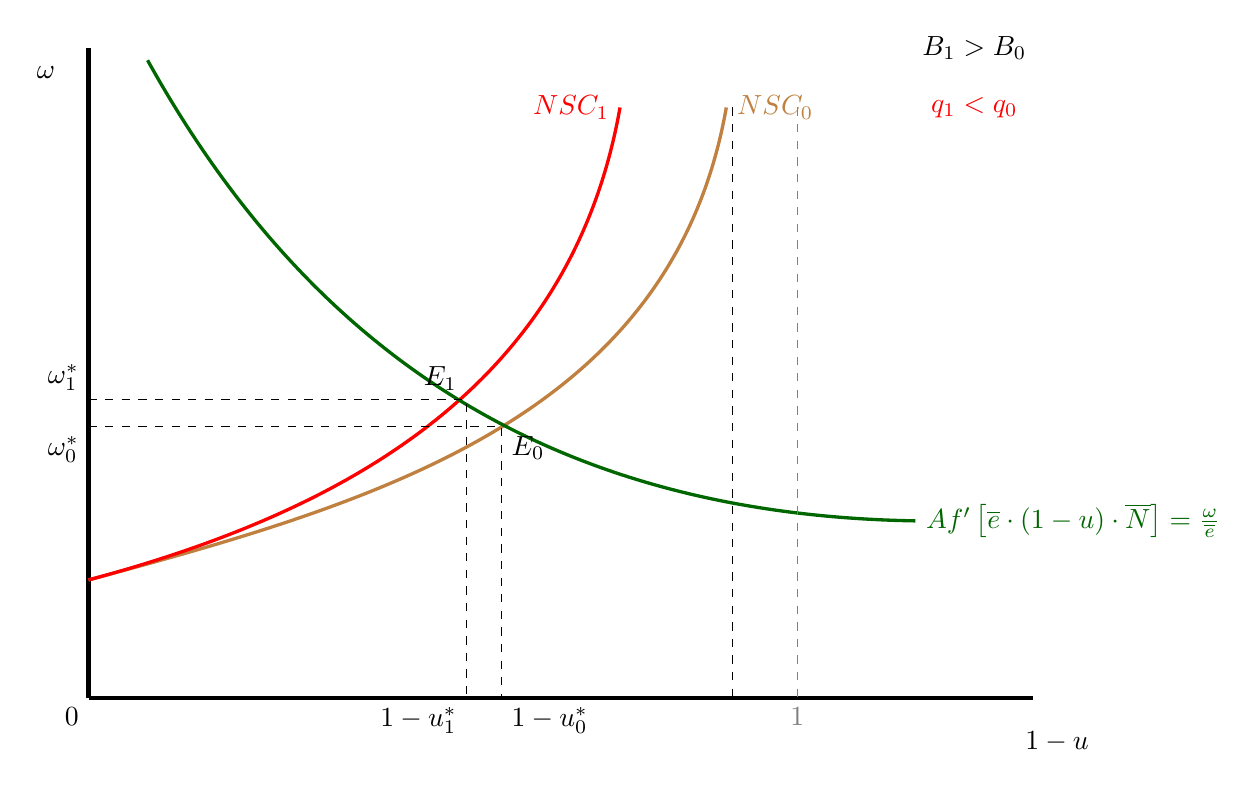
\begin{tikzpicture}[scale=1.5]

% Axis

\draw [ultra thick](0,0) -- (8,0);

\draw [ultra thick](0,0) -- (0,5.5);

\node [left] at (-0.2,5.3) {$\omega$};

\node [below] at (8.2,-0.2) {$1 - u$};
\node [below left] at (0,0) {$0$};

%\node [left] at (0,1) {$\left[ \frac { q B ^ { \alpha } } { ( 1 - \overline { e } ) ^ { 1 - \alpha } - ( 1 - q ) } \right] ^ { \frac { 1 } { \alpha } }$};


%\node[gray] [left] at (0,3.5) {$\left[ \frac { q \cdot \overline { \omega } ^ { \alpha } \cdot ( 1 - \overline { e } ) ^ { 1 - \alpha } } { ( 1 - \overline { e } ) ^ { 1- \alpha } - ( 1 - q ) } \right] ^ { \frac { 1 } { \alpha } }$};

%Curve
\draw[very thick, brown] (0,1) to [out=15,in=260]  (5.4,5) node[right]{$NSC_0$};
\draw[very thick, red] (0,1) to [out=15,in=260]  (4.5,5) node[left]{$NSC_1$};
\draw[very thick, black!60!green] (0.5, 5.4) to [bend right = 30] (7,1.5) node [ right] {$Af ^ { \prime } \left[ \overline { e } \cdot ( 1 - u ) \cdot \overline { N } \right] = \frac { \omega } { \overline { e } }$};

\draw [dashed] (5.45,5)--(5.45,0);

\draw [dashed] (0,2.525) node[above left]{$\omega^*_1$}  -- (3.2,2.525) node[above left]{$E_1$} -- (3.2, 0) node[below left] {$1 - u^*_1$};

\draw [dashed] (0,2.3) node[below left]{$\omega^*_0$} -- (3.5,2.3) node[below right] {$E_0$} -- (3.5, 0) node[below right] {$1 - u^*_0$}  ;


\node at (7.5,5.5) {$B_1 > B_0$};
\node [red] at (7.5,5) {$q_1 < q_0$};


\draw [dashed, gray] (6,5)--(6,0)node[below]{$1$};
\end{tikzpicture}

\caption{Equilibrium and shocks to the NSC}

\end{figure}


A negative shock to q, as in the graph, $q_{1}<q_{0}$ moves the NSC to the left, resulting in a higher real wage for workers, but reducing overall employment. A positive shock to unemployment benefits, as $B_{1}>B_{0}$, moves the right, making the real wage lower, but resulting in more employment.  

\newpage
\subsection{Search and Matching Model}
\subsubsection{The matching function}
\begin{equation}\label{Matching_function}
    M_{t}=M(u_{t}.L_{t},V_{t}.L_{t})
\end{equation}

Define $x=u.L, V.L$

\begin{itemize}
    \item $\frac{\partial M}{\partial x}>0$
    \item $\frac{\partial^{2}M}{\partial x^{2}}<0$
    \item $\frac{\partial^{2}}{\partial(u.L)}\frac{\partial^{2}}{\partial(V.L}-\frac{\partial^{2}M}{\partial(u.L\partial(V.L)}>0$
\end{itemize}

\begin{itemize}
    \item $M(\lambda u.L, \lambda v.L>\lambda M(u.L,V.L) \implies$ Thick market condition
    \item $M(\lambda u.L, \lambda v.L<\lambda M(u.L,V.L) \implies$ Crowding effects
\end{itemize}

\begin{equation*}
\begin{aligned}
    M_{t}=\xi(u_{t}.L_{t})^{1-\eta}(V_{t}L_{t})^{\eta} \\
    M_{t}=\xi u_{t}^{1-\eta}V_{t}^{\eta}L_{t} 
\end{aligned}
\end{equation*}

\begin{equation*}
\begin{aligned}
    m_{t}=\frac{M_{t}}{L_{t}}=\xi u_{t}^{1-\eta}V_{t}^{\eta} \implies v_{t}=\big(\frac{m_{t}}{\xi}\big)^{\frac{1}{\eta}}u_{t}^{-\frac{1-\eta}{\eta}}
\end{aligned}
\end{equation*}
$v_{t}=\big(\frac{m_{t}}{\xi}\big)^{\frac{1}{\eta}}u_{t}^{-\frac{1-\eta}{\eta}}$ is known as the Beveridge curve, and $\frac{m_{t}}{\xi}$ is a measure for the level of frictions in the labour market. 

\subsubsection{Labour-Market flows: Mortensen-Pisserides}
\begin{equation*}
\begin{aligned}
    \Delta N_{t+1}^{*}=M_{t} -\lambda N_{t}^{*} \\
    m_{t}=\xi\big(\frac{V_{t}}{u_{t}}\big)^{\eta}u_{t} \\
    m_{t}=\xi\theta_{t}^{\eta}u_{t}
\end{aligned}  
\end{equation*}

Where $\theta_{t}=\frac{v_{t}L_{t}}{u_{t}l_{t}}=\frac{v_{t}}{u_{t}}$ is the tightness ration.

We can define the job finding rate:
\begin{equation}\label{JFR}
    \phi_{t}=\frac{M_{t}}{u_{t}L_{t}}=\frac{m_{t}}{u_{t}}=\xi \theta_{t}^{\eta}
\end{equation}

And the vacancy filling rate: 
\begin{equation}\label{VFR}
    \beta_{t}=\frac{M_{t}}{u_{t}L_{t}}=...=\xi\theta_{t}^{\eta-1}
\end{equation}

\begin{equation*}
    \frac{\Delta N_{t+1}^{*}}{L_{t}}=m_{t}-\lambda(1-u_{t})=\xi\theta_{t}^{\eta}u_{t}-\lambda(1-u_{t})
\end{equation*}

\subsubsection{Intertemporal Optimization}

\begin{equation*}
    \mathcal{V}_{t}=E_{t}\sum_{\tau=t}^{\infty}(1+\rho)^{-(\tau-t)}.V_{\tau} 
\end{equation*}

\begin{equation*}
    \mathcal{V}_{t}=V_{t}+E_{t}\sum_{\tau=t+1}^{\infty}(1+\rho)^{-(\tau-t)}.V_{\tau} 
\end{equation*}

\begin{equation*}
    \mathcal{V}_{t}=V_{t}+\frac{1}{1+\rho}\sum_{\tau=t+1}^{\infty}(1+\rho)^{-[\tau-(t+1)]}.V_{t} 
\end{equation*}

\begin{equation*}
    \mathcal{V}_{t}=V_{t}+\frac{1}{1+\rho}\mathcal{V}_{t+1}
\end{equation*}

\subsubsection{Firms}
\begin{equation*}
y_{t}=A_{t}.N_{t}-\Phi
\end{equation*}
Firms produce only with labour, and we normalize their number of workers to one, so $N_{t}$ can only be one of two values: 

\[ 
N_{t}=\left\{
\begin{array}{l l}
    1 & \text{position filled (F)}  \\
    0 & \text {position vacant (V)}
\end{array}
\right.
\]
And so profits can also take one of only two values: 
\[ 
\pi_{t}=\left\{
\begin{array}{cc}
    \pi_{t}^{F}=A_{t}-\Phi-\omega_{t} & N_{t}=1  \\
     \pi_{t}^{V}=-\Phi & N_{t}=0 
\end{array}
\right.
\]

\begin{enumerate}
    \item $\mathcal{V}_{t}^{F}=\pi_{t}^{F}+\frac{1}{1+\rho}\bigg[(1-\lambda)\mathcal{V}_{t+1}^{F}+\lambda\mathcal{V}_{t+1}^{V} \bigg]$
    \item $\mathcal{V}_{t}^{V}=\pi^{V}_{t}=\frac{1}{1+\rho}\bigg[(1+\beta_{t+1})\mathcal{V}_{t+1}^{V}+\beta_{t+1}\mathcal{V}_{t+1}^{F} \bigg]$
\end{enumerate}

\subsubsection{Households}
\[ 
U_{t}=\left\{
\begin{array}{l l}
     U_{t}^{E}=\omega_{t} & L_{t}=1  \\
     U_{t}^{U}=B & L_{t}=0 
\end{array}
\right.
\]

$B< min [\omega_{t}, A_{t}]$

\begin{enumerate}
    \item $\mathcal{V}_{t}^{E}=\omega_{t}+\frac{1}{1+\rho}\bigg[ (1-\lambda)\mathcal{V}_{t+1}^{E}+\lambda\mathcal{V}_{t+1}^{U} \bigg] $, where, $\omega_{t}=U_{t}^{E}$
    \item $\mathcal{V}_{t}^{U}=B+\frac{1}{1+\rho}\bigg[ (1-\phi_{t+1})\mathcal{V}_{t+1}^{U}+\phi_{t+1}\mathcal{V}_{t+1}^{E} \bigg] $
\end{enumerate}

\subsubsection{Bargaining}
\begin{equation*}
\begin{aligned}
    \underset{{\mathcal{P}^{V}},\mathcal{P}^{U}}{max} & (\mathcal{V}_{t}^{F}-\mathcal{V}_{t}^{V})^{\varepsilon}(\mathcal{V}_{t}^{E}-\mathcal{V}_{t}^{U})^{1-\varepsilon} \\
    s.t. & \mathcal{P}^{V}+\mathcal{P}^{U}=\mathcal{P}_{t}
\end{aligned}
\end{equation*}
Note that $\mathcal{V}_{t}^{F}-\mathcal{V}_{t}^{V}=\mathcal{P}^{V}$, and, $\mathcal{V}_{t}^{E}-\mathcal{V}_{t}^{U}=\mathcal{P}^{U}$.
\paragraph{} 
From the first order conditions we get the Nash bargaining solution: 

\begin{equation}\label{Nas_Barg_Solution}
    \frac{\mathcal{P}_{t}^{U}}{\mathcal{P}_{t}^{V}}=\frac{1-\varepsilon}{\varepsilon}
\end{equation}

\subsubsection{Steady State}
We evaluate the system dynamics only at a steady state. For this purpose we'll compute the variables at a steady state. 

\begin{equation*}
    \Delta N_{t+1}^{*}=0 \implies o=\xi . \theta^{\eta}.u-\lambda(1-u) \implies u=\frac{\lambda}{\lambda + \xi.\theta^{\eta}}
\end{equation*}

Note: $\xi.\theta^{\eta}=\phi$ which is the Job finding rate. 

\begin{equation*}
\begin{aligned}
    \mathcal{V}^{V}=-\frac{1+\rho}{\rho+\beta}.\Phi+\frac{\beta}{\rho+\beta}.\mathcal{V}^{F} \\
    + \\
    \mathcal{V}^{F}=\frac{(1+\rho)(\rho+\beta)}{\rho(\rho+\beta+\lambda)}(A-\omega)-\frac{1+\rho}{\rho}\Phi \\ 
    = \\
    \mathcal{V}^{V}=-\frac{1+\rho}{\rho}.\Phi+\frac{\beta(1+\rho)}{\rho(\rho+\beta+\lambda)}(A-\omega) \\
   \implies \mathcal{P}^{V}=\mathcal{V}^{F}-\mathcal{V}^{V}=...=\frac{1-\rho}{\rho+\lambda+\beta}(A-\omega)
\end{aligned}
\end{equation*}

\begin{equation*}
\begin{aligned}
    \mathcal{V}^{E}=\frac{1+\rho}{\rho+\lambda}\omega+\frac{\lambda}{\rho+\lambda}\mathcal{V}^{U} \\ 
    + \\
    \mathcal{V}^{U}=\frac{(1+\rho)(\rho+\lambda)}{\rho+(\rho+\lambda+\phi<)} \\
    = \\
    \mathcal{V}^{E}=\frac{(1+\rho)(\rho+\phi)}{\rho(\rho+\lambda+\phi)}\omega+ \frac{\lambda(1+\rho)}{\rho(\rho+\lambda+\phi)}B \\
    \implies \mathcal{P}^{U}=\mathcal{V}^{E}-\mathcal{V}^{U}=...=\frac{1+\rho}{\rho+\lambda+\phi}(\omega-B)
\end{aligned}
\end{equation*}
We can now introduce these expressions in the Nash Bargaining Solution \ref{Nas_Barg_Solution};

\begin{equation*}
\begin{aligned}
    \frac{\mathcal{P}^{U}}{\mathcal{P}^{V}}=\frac{1-\varepsilon}{\varepsilon} \\
    \implies \omega=B+\frac{(1-\varepsilon)(\rho+\lambda+\phi)}{\rho+\lambda+(1-\varepsilon)\phi+\varepsilon\beta}
\end{aligned}
\end{equation*}

For $\phi=\beta \implies \omega-B=(1-\varepsilon)(A-B)$. Also, $\frac{\partial(\omega-B)}{\partial\beta}<0$.

\begin{equation*}
    \mathcal{V}^{V}=...=-\frac{1+\rho}{\rho}\Phi+\frac{\beta(1+\rho)\varepsilon}{\rho \big[\rho+\lambda+\phi(1-\varepsilon)+\varepsilon\beta \big]}(A-B)
\end{equation*}

\begin{equation*}
    u=\frac{\lambda}{\lambda +\xi\theta^{\eta}} \implies \theta=\bigg[\frac{\lambda(1-u)}{\xi u} \bigg]^{\frac{1}{\eta}}
\end{equation*}

Recall that $\beta$ in \ref{JFR} is the job finding rate (JFR), and $\phi$ in \ref{VFR} is the vacancy filling rate (VFR). 
\begin{equation*}
    \beta=\xi \bigg[\frac{\lambda(1-u)}{\xi u} \bigg]^{\frac{\eta-1}{\eta}} \implies \frac{\partial\beta}{\partial u}>0
\end{equation*}

\begin{equation*}
    \theta=\xi\frac{\lambda(1-u)}{\xi u} \implies \frac{\partial \phi}{\partial u}<0
\end{equation*}

\begin{equation*}
    \begin{aligned}
        \mathcal{V}^{V}=-\frac{\rho+1}{\rho}.\Phi+\frac{1+\rho}{\rho}\frac{\varepsilon\beta(u)}{\rho+\lambda+(1-\varepsilon)\phi(u)+\varepsilon\beta(u)}
    \end{aligned}
\end{equation*}
\begin{equation*}
     \mathcal{V}^{V}=-\frac{1+\rho}{\rho}\Phi+h(u)
\end{equation*}
$h'(u)>0$

\subsubsection{Free entry}
\begin{equation*}
    \mathcal{V}^{V}=0
\end{equation*}
\begin{equation*}
    0=-\frac{1+\rho}{\rho}.\Phi+h(u) \implies u^{*}=h^{-1}\big(\frac{1+\rho}{\rho}\Phi
\end{equation*}

\subsubsection{Changes in Productivity and Unemployment benefits}
\begin{equation*}
    \frac{\partial h}{\partial(A-B)}>0
\end{equation*}

\subsubsection{Welfare}
$L_{t}=L_{0}$

\begin{equation*}
    \frac{\Delta N_{t+1}}{L_{t}}=\frac{N_{t+1}^{*}-N_{t}^{*}}{L_{0}}=\frac{(1-u_{t-1})L_{0}-(1-u_{t})L_{0}}{L_{0}}=-\Delta u_{t+1}
\end{equation*}

\begin{equation*}
    \begin{aligned}
        \underset{u_{t},V_{t}}{max}\sum_{\tau=t}^{\infty}(1+\rho)^{-(\tau-t)}\bigg[(A_{t}-\Phi)(1-u_{t})+Bu_{t}-\Phi V_{t} \bigg] \\
    &   s.t. \Delta u_{t+1}=\lambda (1-u_{t}) - \xi V_{t}^{\eta}u_{t}^{1-\eta}
    \end{aligned}
\end{equation*}

\begin{equation*}
    H=(A_{t}-\Phi)(1-u_{t})+Bu_{t}-\Phi V_{t}+\mu_{t}\big[\lambda(1-u_{t})-\xi u_{t}^{1-\eta}V_{t}^{\eta} \big]
\end{equation*}

\begin{enumerate}
    \item $\frac{\partial H}{\partial V}= 0 \implies -\Phi-\mu_{t}\eta\xi u_{t}^{1-\eta} V_{t}^{\eta-1}=0$
    \item $\frac{\partial H}{\partial u}=0 \implies -(A_{t}-\Phi)+B-\mu_{t}\lambda u_{t}(1-\eta)\xi\mu_{t}^{-\eta}V_{t}^{\eta}=0$
\end{enumerate}

\begin{enumerate}
    \item $\mu.\eta.\xi.\big(\frac{V}{u}\big)^{\eta-1}=-\Phi \implies \mu=\frac{-\Phi}{\eta\beta}$. Note that $\frac{V}{u}=\theta$, and $\xi\big(\frac{V}{u}\big)^{\eta-1}=\beta(\theta)$ 
    \item $-(A-\Phi-B)=\big[\rho+\lambda+(1-\eta).\xi.(\frac{V}{u})^{\eta} \big].\mu \implies A-B=\frac{\lambda+\rho+(1+\eta).\phi+\eta.\beta}{\eta.\beta}.\Phi$. This gives us the Welfare-Maximizing solution for the central planner.
\end{enumerate}

\begin{equation*}
    \begin{aligned}
        \mathcal{V}^{V}=0 \\ \implies-\frac{1+\rho}{\rho}.\Phi+\frac{1+\rho}{\rho}.(a-B).\frac{\varepsilon\beta}{\lambda+\rho+(1-\varepsilon)\phi+\varepsilon\beta}=0 \\
        \implies A-B=\frac{\lambda+\rho+(1-\varepsilon)\Phi+\varepsilon\beta}{\varepsilon.\beta}.\Phi 
    \end{aligned}
\end{equation*}
Which is the decentralized equilibrium. 
\paragraph{} 
We can see the two are different, except for the case of $\eta=\varepsilon$ (Hosios solution), which is a very specific and sensitive situation, where a small deviation in one of the variables will put the economy in a different equilibrium. 




